
\section{IaaS Service Ontology}
\label{chap:ontology}

What is an otlology? An ontology is a specification of a conceptualization. According to Gruber \cite{OntologyDefinition} an ontology defines a set of representational primitives with which to model a domain of knowledge. These  primitives are typically classes (or sets), attributes (or properties), and relationships (or relations among class members). The definitions of the representational primitives include information about their meaning and constraints on their logically consistent application.

% http://tomgruber.org/writing/ontology-definition-2007.htm
% http://www.opengroup.org/soa/source-book/ontologyv2/intro.htm#fig_soa_ontology

% ontologie jine fieldy - medicina

% zkratit

There formal definition of cloud comptuting architecture 

\begin{figure}[!h]
\centering
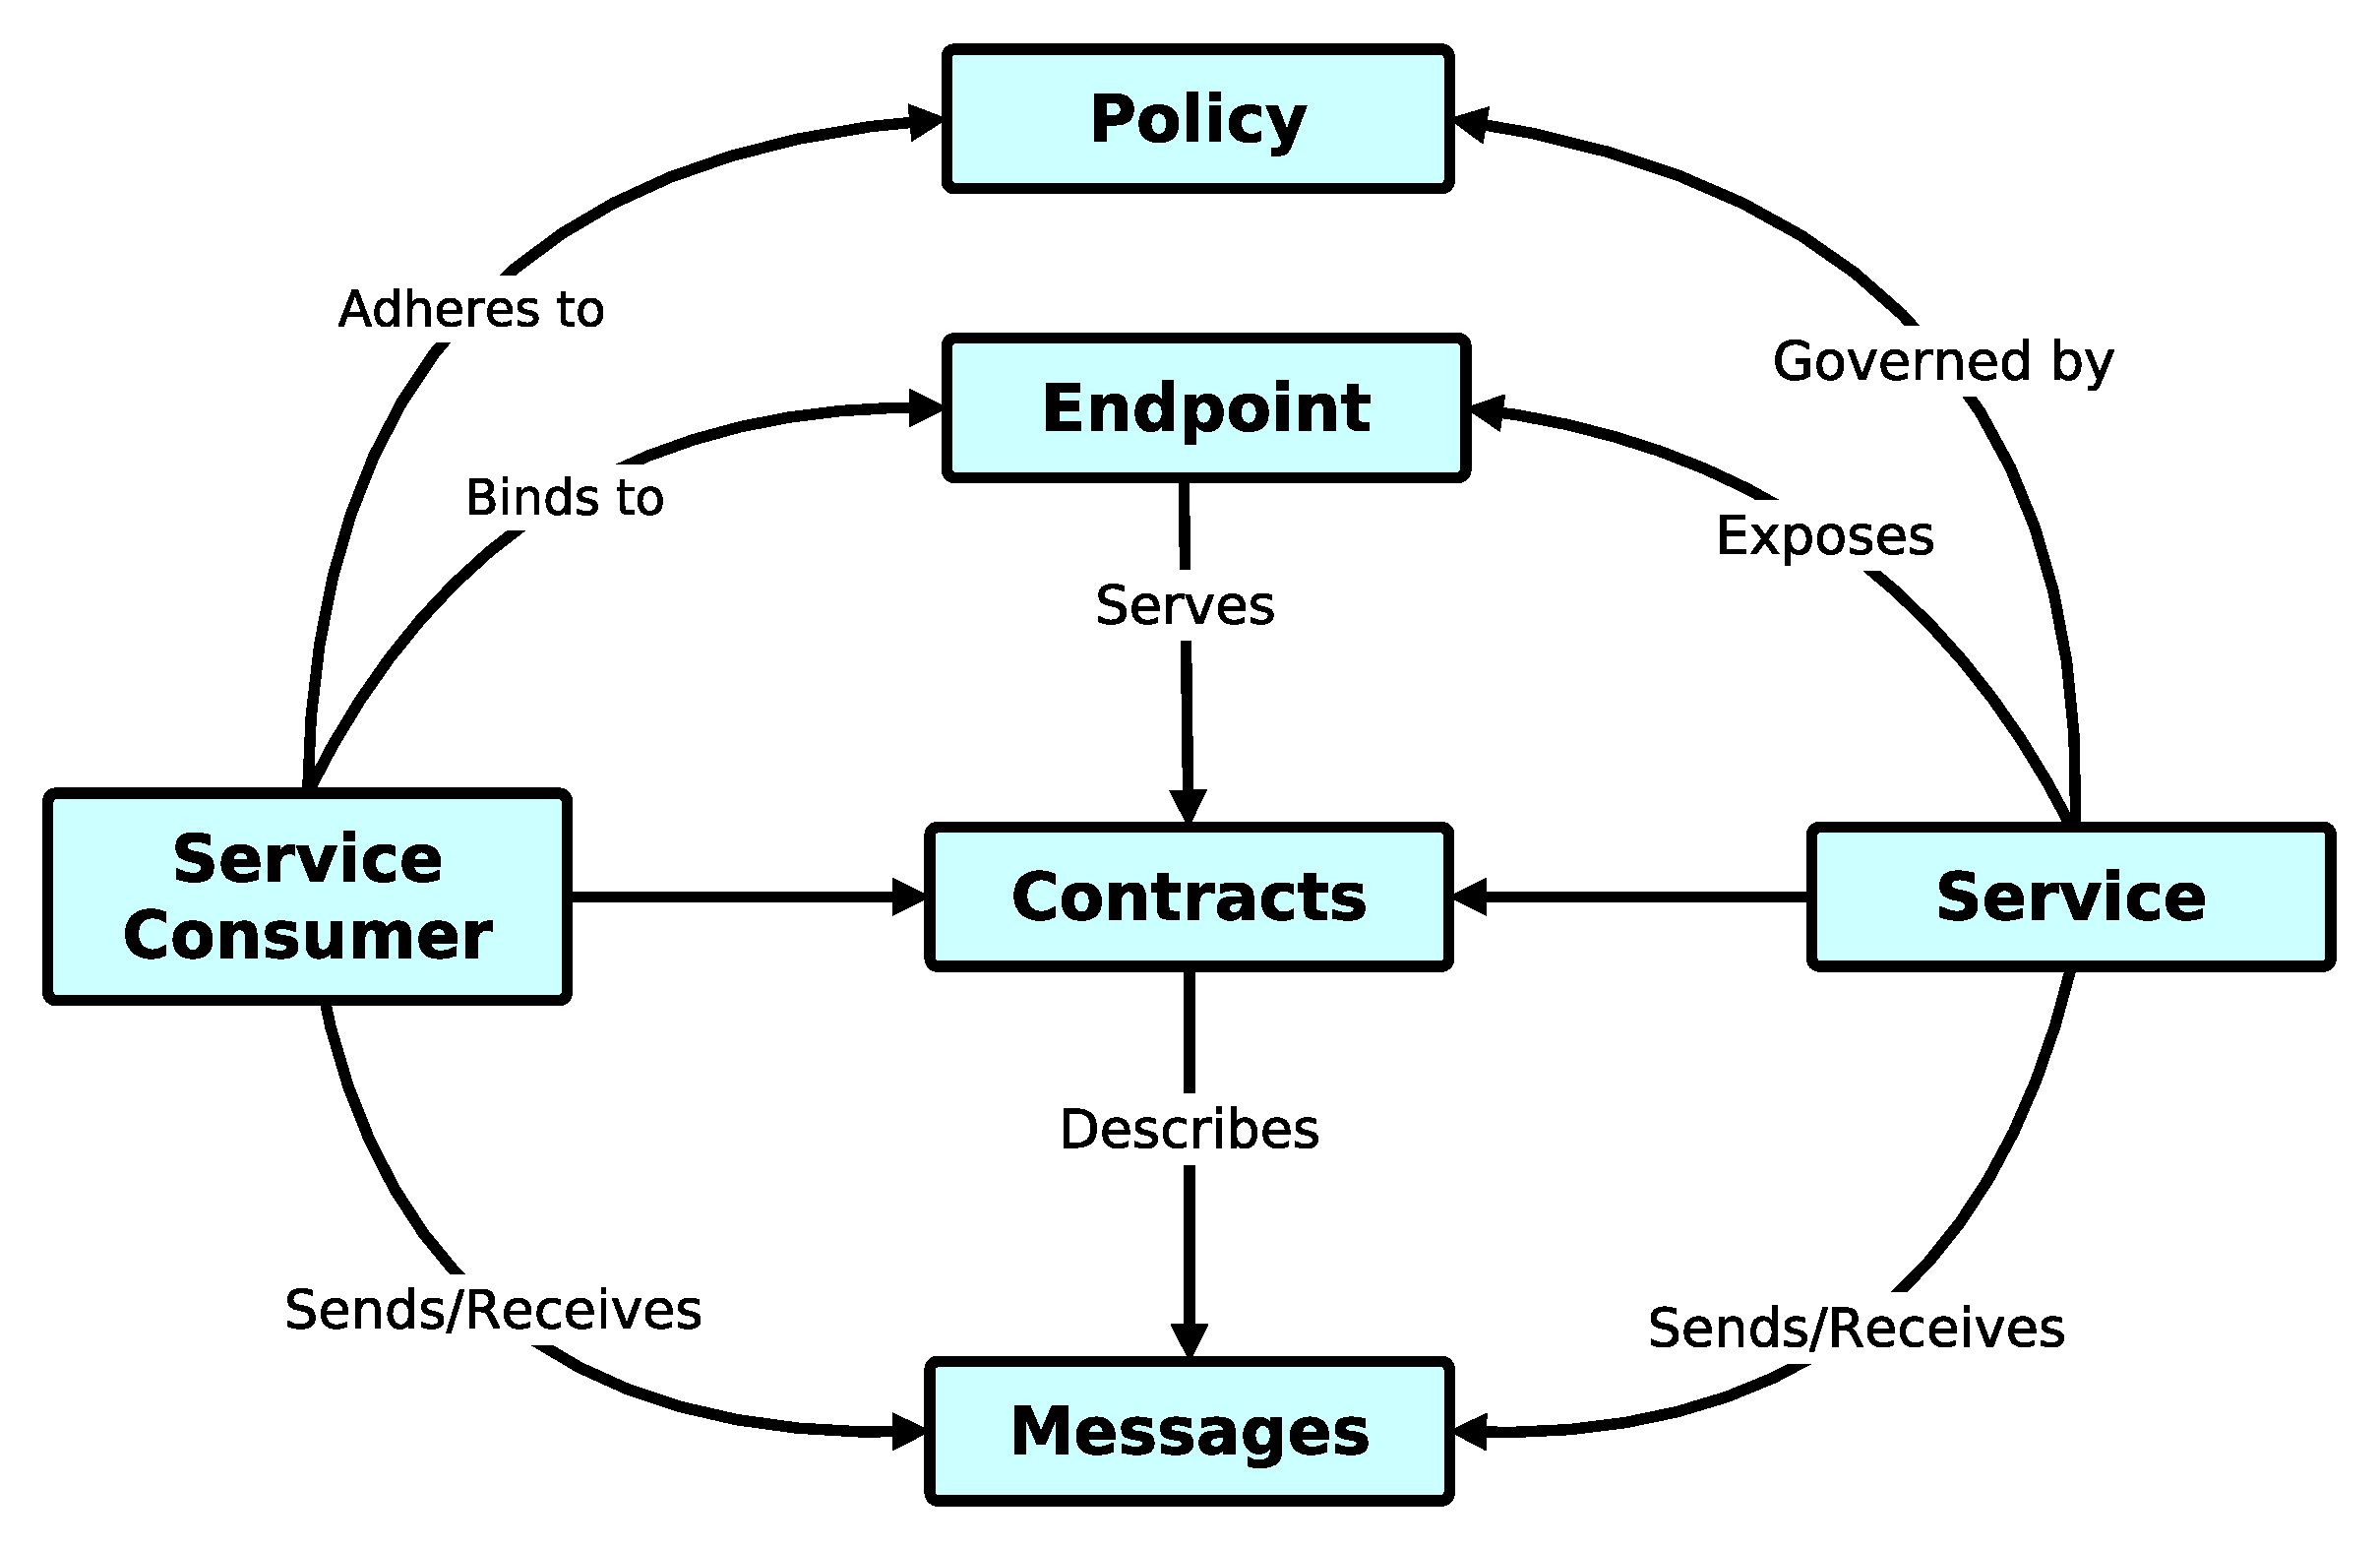
\includegraphics[scale=.2]{img/soa_relation.eps}
\caption{SOA Sbject Property Service Interface}
\label{fig:cm}
\end{figure}

1. Servers (physical and virtual)

2. Core Infrastructure Services (DNS, DHCP, NTP, image management)

3. Storage (NAS and SAN)

4. Network (Routers, Switches, Firewalls, Load Balancers)

5. Facilities (Power, Cooling, Space)

\subsection{Ontological Standards}

The ontologies define the relations between terms, but does not prescribe exactly how they should be applied. 

OWL has three increasingly expressive sub-languages: OWL-Lite, OWL-DL, and OWL-Full [OWL]. The sub-language OWL-DL provides the greatest expressiveness possible while retaining computational completeness and decidability.

\subsubsection{Service-Oriented Architecture}

The SOA ontology specification was developed in order to aid understanding, and potentially be a basis for model-driven implementation of software systems

The ontology is represented in the Web Ontology Language (OWL) defined by the World-Wide Web Consortium (W3C). 

The ontology contains classes and properties corresponding to the core concepts of SOA. The formal OWL definitions are supplemented by natural language descriptions of the concepts, with graphic illustrations of the relations between them, and with examples of their use. For purposes of exposition, the ontology also include.

\subsubsection{OSLC Configuration Management}


\subsubsection{Dublin Core Metadata Initiative}

\subsubsection{Basic Formal Ontology}

The Basic Formal Ontology (BFO) is a formal ontological framework developed by Barry Smith and his associates that consists in a series of sub-ontologies at different levels of granularity. The ontologies are divided into two varieties:
 Continuant (or snapshot) ontologies, comprehending continuant entities such as three-dimensional enduring objects, and occurrent ontologies, comprehending processes conceived as extended through (or as spanning) time.

\subsection{Ontology Serialization Formats}

There are many ways how to serialize ontology.

In it's core ontology representation is set of graph edges connecting subject and object vertices.

The 

%- speed - parsing / scaling

%- integration, maintenance costs

%- security issues


\subsubsection{XML Documents}

RDF is a standard model for data interchange on the Web. RDF has features that facilitate data merging even if the underlying schemas differ, and it specifically supports the evolution of schemas over time without requiring all the data consumers to be changed.

RDF extends the linking structure of the Web to use URIs to name the relationship between things as well as the two ends of the link (this is usually referred to as a “triple”). Using this simple model, it allows structured and semi-structured data to be mixed, exposed, and shared across different applications. 

This linking structure forms a directed, labeled graph, where the edges represent the named link between two resources, represented by the graph nodes. This graph view is the easiest possible mental model for RDF and is often used in easy-to-understand visual explanations. 

% http://www.w3.org/RDF/

\subsubsection{Graph databases}

Graph databases can map OWL based ontologies very well as they have format very similar to RDF format which is standard format of any XML based graph database, just very different implementation. Graph database uses graph structures with nodes, edges, and properties to represent and store data. A graph database is any storage system that provides index-free adjacency.This means that every element contains a direct pointer to its adjacent elements and no index lookups are necessary.

% http://en.wikipedia.org/wiki/Graph_database

je to servica, tzn overhead oproti xml filu, ale zas ma api atd ...

\subsection{Plain Meta-data Serialization Formats}

It's tree structure

\subsubsection{Hierarchical Databases}

Subject (id) or property driven

reclass allows you to define your nodes through class inheritance, while always able to override details further up the tree (i.e. in more specific nodes). Think of classes as feature sets, as commonalities between nodes, or as tags. Add to that the ability to nest classes (multiple inheritance is allowed, well-defined, and encouraged), and you can assemble your infrastructure from smaller bits, eliminating duplication and exposing all important parameters to a single location, logically organised. And if that isn’t enough, reclass lets you reference other parameters in the very hierarchy you are currently assembling.

% http://reclass.pantsfullofunix.net/

\subsection{Ontology structure}

\begin{figure}[!h]
\centering
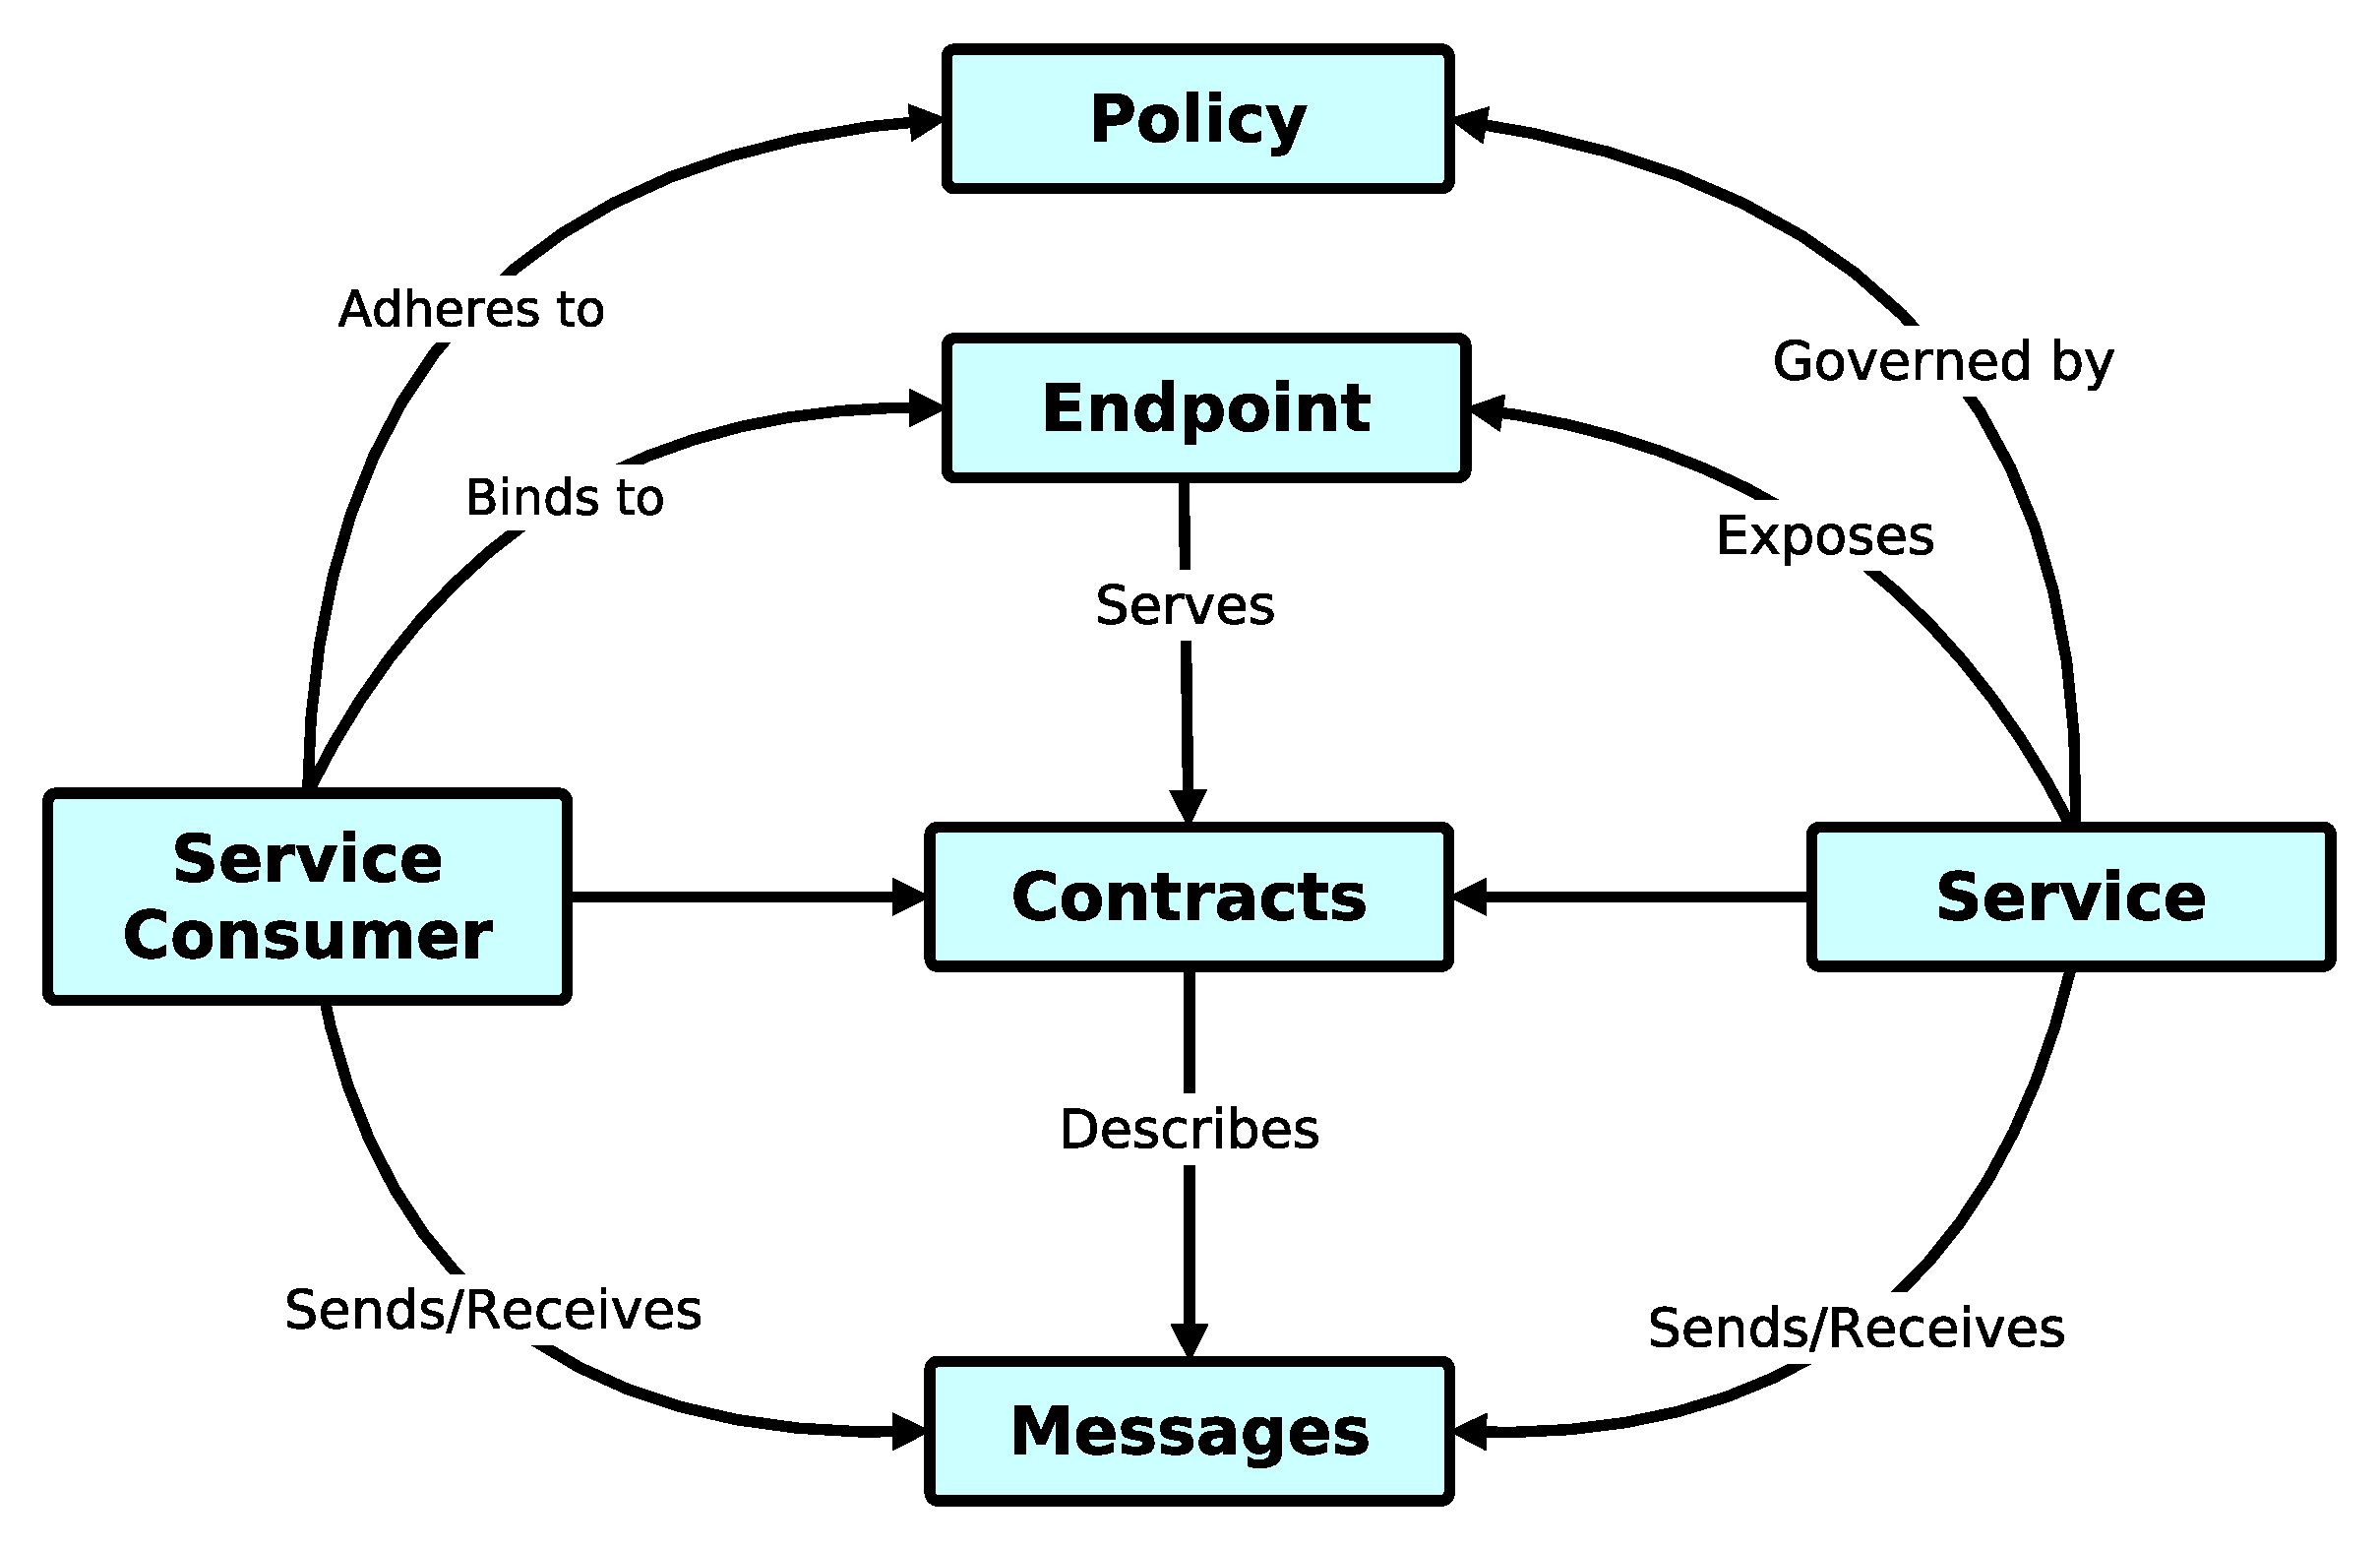
\includegraphics[scale=.2]{img/soa_relation.eps}
\caption{SOA Sbject Property Service Interface}
\label{fig:cm}
\end{figure}

%\begin{figure}[!h]
%\centering
%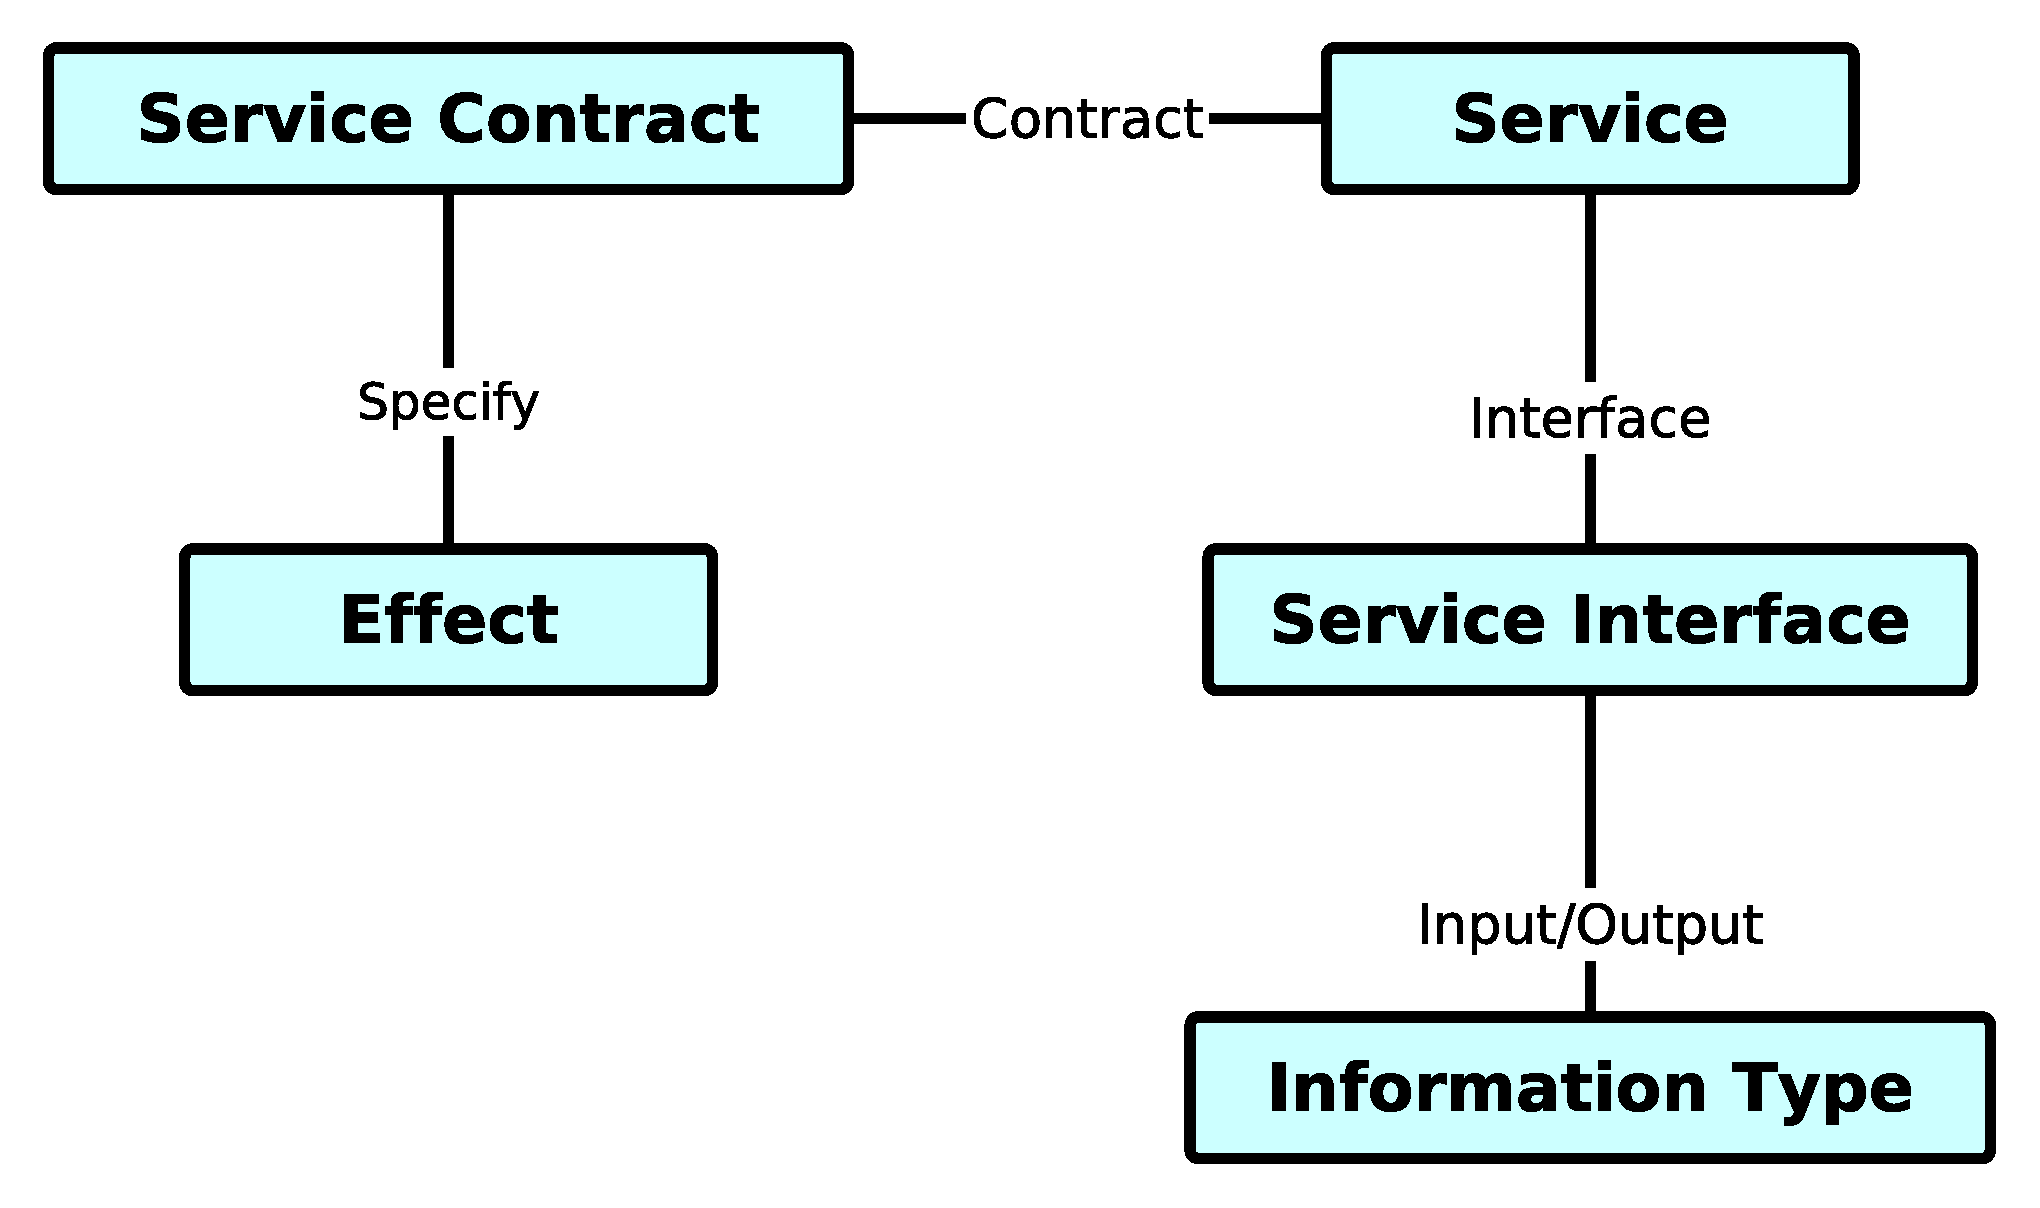
\includegraphics[scale=.2]{img/soa_property.eps}
%\caption{SOA service property}
%\label{fig:cm}
%\end{figure}


%\subsection{Comparison}

% Srovnání jednolivých formátů pro ontologii pro openstack řešení - bezpečnost, rychlost, integrace

